\documentclass{article}
\usepackage{pgfplots}
\begin{document}
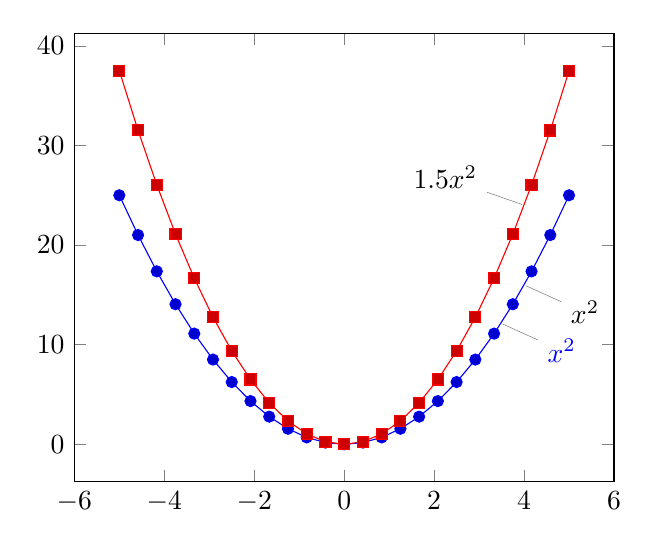
\begin{tikzpicture}
  \begin{axis}
    \addplot {x^2} node [pos=0.75,pin={-10:$x^2$},inner sep=0pt] {}; % This does not position the node on the line
    \addplot {1.5*x^2};
    \node at (axis cs:4,16) [pin={-10:$x^2$},inner sep=0pt] {}; % This is what I want, but without calculating the coordinates by hand
    \node at (axis cs:4,24) [pin={170:$1.5 x^2$},inner sep=0pt] {};
  \end{axis}
\end{tikzpicture}
\end{document}
